\documentclass[conference]{IEEEtran}
\IEEEoverridecommandlockouts
% The preceding line is only needed to identify funding in the first footnote. If that is unneeded, please comment it out.
\usepackage{cite}
\usepackage{amsmath,amssymb,amsfonts}
\usepackage{algorithmic}
\usepackage{graphicx}
\usepackage{textcomp}
\usepackage{xcolor}
\usepackage{tikz}
\usetikzlibrary{shapes,arrows,positioning,fit,calc}
\def\BibTeX{{\rm B\kern-.05em{\sc i\kern-.025em b}\kern-.08em
    T\kern-.1667em\lower.7ex\hbox{E}\kern-.125emX}}
\begin{document}

\title{Partisan Discourse on X: An Analysis of Political Polarization in Social Media\\
}

\author{\IEEEauthorblockN{Ziv Barretto}
\IEEEauthorblockA{\textit{Ashoka University} \\
}
\and
\IEEEauthorblockN{Agriya Yadav}
\IEEEauthorblockA{\textit{Ashoka University} \\
}
\and
\IEEEauthorblockN{Kyra Chhetri}
\IEEEauthorblockA{\textit{Ashoka University} \\
}
\and
\IEEEauthorblockN{Anirban Sen}
\IEEEauthorblockA{\textit{Ashoka University} \\
}
}

\maketitle

\begin{abstract}

\end{abstract}

\begin{IEEEkeywords}
\end{IEEEkeywords}

\section{Introduction}
The rise of social media platforms has fundamentally transformed political communication and discourse. X (formerly known as Twitter) has emerged as a critical platform for political discussion, serving as a space where politicians, journalists, activists, and citizens engage in real-time conversations about political issues. However, this democratization of political discourse has coincided with growing concerns about political polarization and the formation of ideological echo chambers.

This paper investigates partisan discourse on X, examining how political identities and affiliations shape online communication patterns. 
\section{Literature Review}

\section{Methodology}
\subsection{Data Cleaning and Formatting}
To analyze partisan discourse, we first established a ground-truth dataset of partisan affiliations. We utilized a dataset of tweets where the \texttt{retweet\_author} was a known political figure. We employed a mapping file to assign a political party to each \texttt{retweet\_author}.

We then classified these parties into two main blocs: ``Ruling'' (e.g., BJP, NDA, JDU) and ``Opposition'' (e.g., INC, TMC, SP). To determine the partisan leaning of the original authors (the ``influencers'' whose content was retweeted), we calculated a yearly polarity score ($P_{yearly}$) for each author based on the volume of retweets they received from politicians of each bloc:
\begin{equation}
P_{yearly} = \frac{R - O}{R + O}
\end{equation}
where $R$ is the count of retweets from Ruling party members and $O$ is the count from Opposition members.

We then computed an average polarity score ($P_{avg}$) across all available years for each author. Based on this score, authors were classified as:
\begin{itemize}
    \item \textbf{Pro-Ruling}: $P_{avg} \ge 0.5$
    \item \textbf{Pro-Opposition}: $P_{avg} \le -0.5$
    \item \textbf{Neutral}: $-0.5 < P_{avg} < 0.5$
\end{itemize}
This classification allowed us to label the original tweets in our dataset with a ``Pro-Ruling'', ``Pro-Opposition'', or ``Neutral'' tag based on the affiliation of their author.

\subsection{Fine-tuning and Stance Detection Model}
To classify the stance of tweets towards specific entities (keywords), we employed a Few-Shot Stance Classification approach enhanced with Low-Rank Adaptation (LoRA). We utilized a pre-trained Large Language Model (LLM) as the base model.

A critical component of our approach is the dynamic retrieval of few-shot examples. For each target keyword (entity), we maintain a specific set of labeled examples (stored as JSON files). During inference, the system reads the keyword associated with a tweet and retrieves the corresponding few-shot examples from the database. If specific examples for a keyword are unavailable, the system falls back to a global set of examples. This ensures that the model receives contextually relevant guidance for each classification task.

The model was adapted using LoRA, a parameter-efficient fine-tuning technique that freezes the pre-trained model weights and injects trainable rank decomposition matrices into each layer of the Transformer architecture. This allowed us to adapt the model to the specific task of political stance detection without the computational cost of full fine-tuning.

\subsection{Stance Detection Process}
The stance detection pipeline was designed to process tweets in batches. For each tweet, we constructed a prompt that included:
\begin{enumerate}
    \item A task description defining stance classification (Support, Deny, Neutral, Unrelated).
    \item A set of few-shot examples provided in JSON format to guide the model's output structure.
    \item The target entity (keyword) and the tweet text.
\end{enumerate}

The model was constrained to generate a valid JSON object containing two keys: ``stance'' (the predicted label) and ``reason'' (a brief explanation). We employed a custom inference pipeline that handled tokenization, batched generation, and robust JSON parsing. To ensure consistency, the model's output labels were normalized to a standard set: ``supports'' (mapped to ``For''), ``denies'' (mapped to ``Against''), ``neutral'', and ``unrelated''. This structured approach ensured high-quality, interpretable stance labels for our large-scale dataset.

\begin{figure}[htbp]
\centering
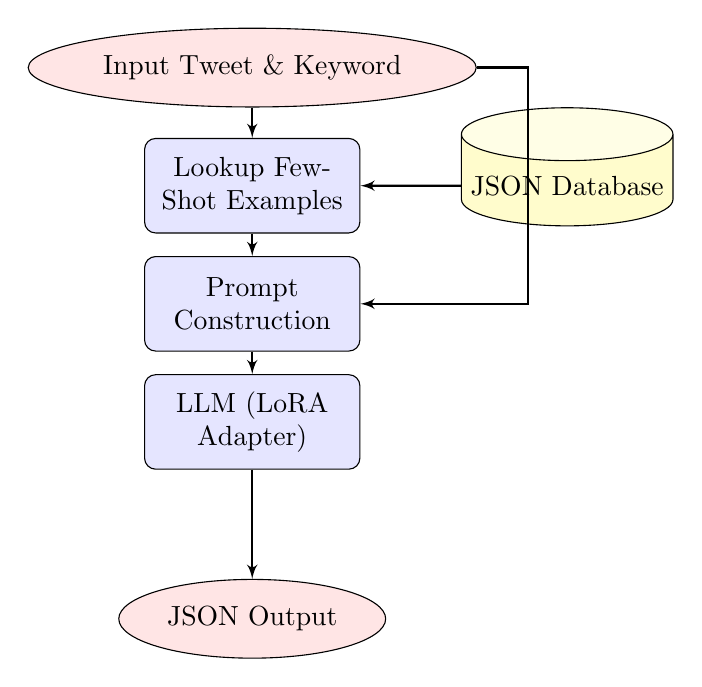
\begin{tikzpicture}[
    node distance=1.5cm,
    auto,
    block/.style={
        rectangle,
        draw,
        fill=blue!10,
        text width=2.5cm,
        text centered,
        rounded corners,
        minimum height=1.2cm
    },
    cloud/.style={
        draw,
        ellipse,
        fill=red!10,
        node distance=2.5cm,
        minimum height=1cm
    },
    decision/.style={
        diamond,
        draw,
        fill=green!10,
        text width=1.5cm,
        text centered,
        inner sep=0pt
    },
    database/.style={
        cylinder,
        cylinder uses custom fill,
        cylinder body fill=yellow!20,
        cylinder end fill=yellow!10,
        shape border rotate=90,
        draw,
        aspect=0.25,
        minimum height=1.5cm,
        text centered
    },
    line/.style={
        draw,
        -latex',
        thick
    }
]

% Nodes
\node [cloud] (input) {Input Tweet \& Keyword};
\node [block, below of=input] (lookup) {Lookup Few-Shot Examples};
\node [database, right of=lookup, node distance=4cm] (db) {JSON Database};
\node [block, below of=lookup] (prompt) {Prompt Construction};
\node [block, below of=prompt] (llm) {LLM (LoRA Adapter)};
\node [cloud, below of=llm] (output) {JSON Output};

% Edges
\path [line] (input) -- (lookup);
\path [line] (db) -- (lookup);
\path [line] (lookup) -- (prompt);
\path [line] (input) -- ++(3.5,0) |- (prompt);
\path [line] (prompt) -- (llm);
\path [line] (llm) -- (output);

\end{tikzpicture}
\caption{Architecture of the Stance Detection System. The system retrieves keyword-specific few-shot examples to construct a prompt, which is then processed by the LoRA-adapted LLM to generate a structured JSON output.}
\label{fig:architecture}
\end{figure}

\section{Results}
\subsection{Partisan Network Structure}

\subsection{Content Characteristics}

\subsection{Interaction Patterns}

\subsection{Temporal Dynamics}

\section{Discussion}

\section{Conclusion}

\section*{Acknowledgment}
We would like to thank Ashoka University for supporting this research.

\begin{thebibliography}{00}
\bibitem{b1} Author, A. A., Author, B. B., and Author, C. C. ``Title of the paper,'' \textit{Journal Name}, vol. X, no. Y, pp. ZZ-ZZ, Month Year.
\bibitem{b2} Author, D. D. ``Title of another paper,'' in \textit{Proceedings of Conference Name}, City, Country, Year, pp. XX-XX.
\bibitem{b3} Author, E. E. and Author, F. F. ``Yet another paper title,'' \textit{Journal Name}, vol. X, no. Y, pp. ZZ-ZZ, Month Year.
\end{thebibliography}

\end{document}
